\item Dibujar la región limitada por las curvas y calcular su área.
\begin{multicols}{2}
  \begin{enumerate}
    \item $\D y= \sqrt x$,\quad $\D y= x^2$.
    \item $\D y= 8-x^2$,\quad $\D y= x^2 $.
    \item $\D y= 5-x^2$,\quad $\D y= 3-x $.
    \item $\D y^2=2x$,\quad $\D x-y=4  $.
    \item $\D x-y^2+3=0 $,\quad $\D x-2y=0  $.
  \end{enumerate}
  
\end{multicols}

\item Para cada dibujo, escribir el área de la región sombreada como una suma de integrales.

\begin{center}
  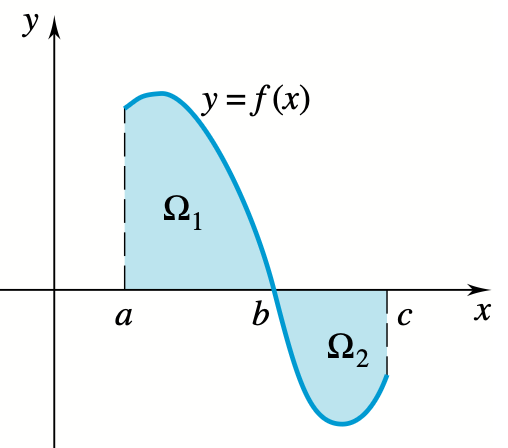
\includegraphics[height=.22\textwidth]{pics/areas-7a.png}
  \hfil
  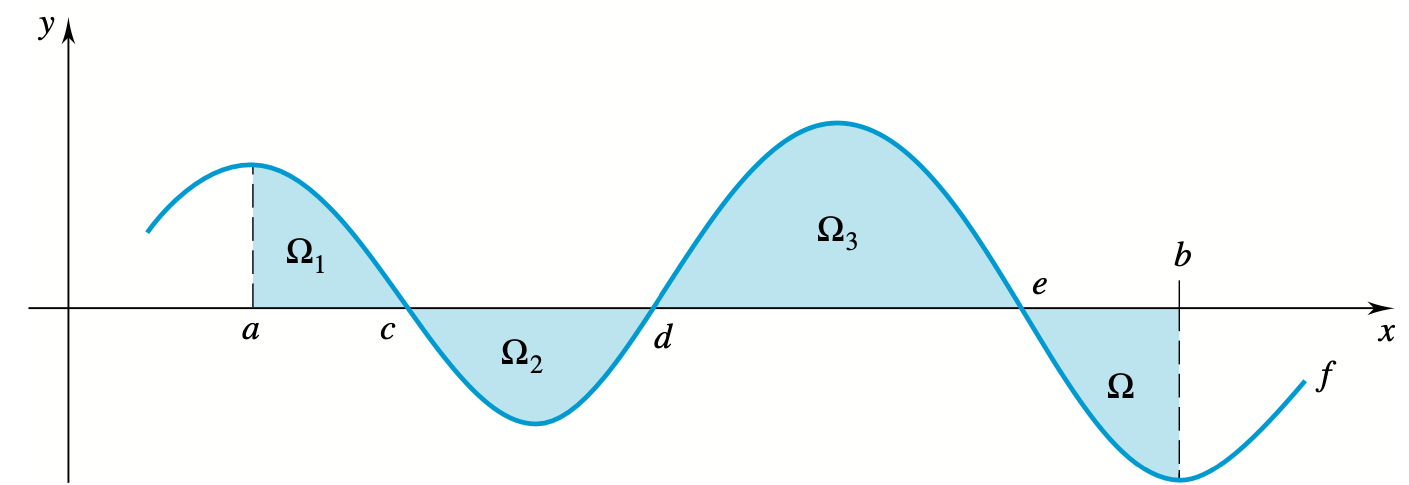
\includegraphics[height=.22\textwidth]{pics/areas-7b.png}

  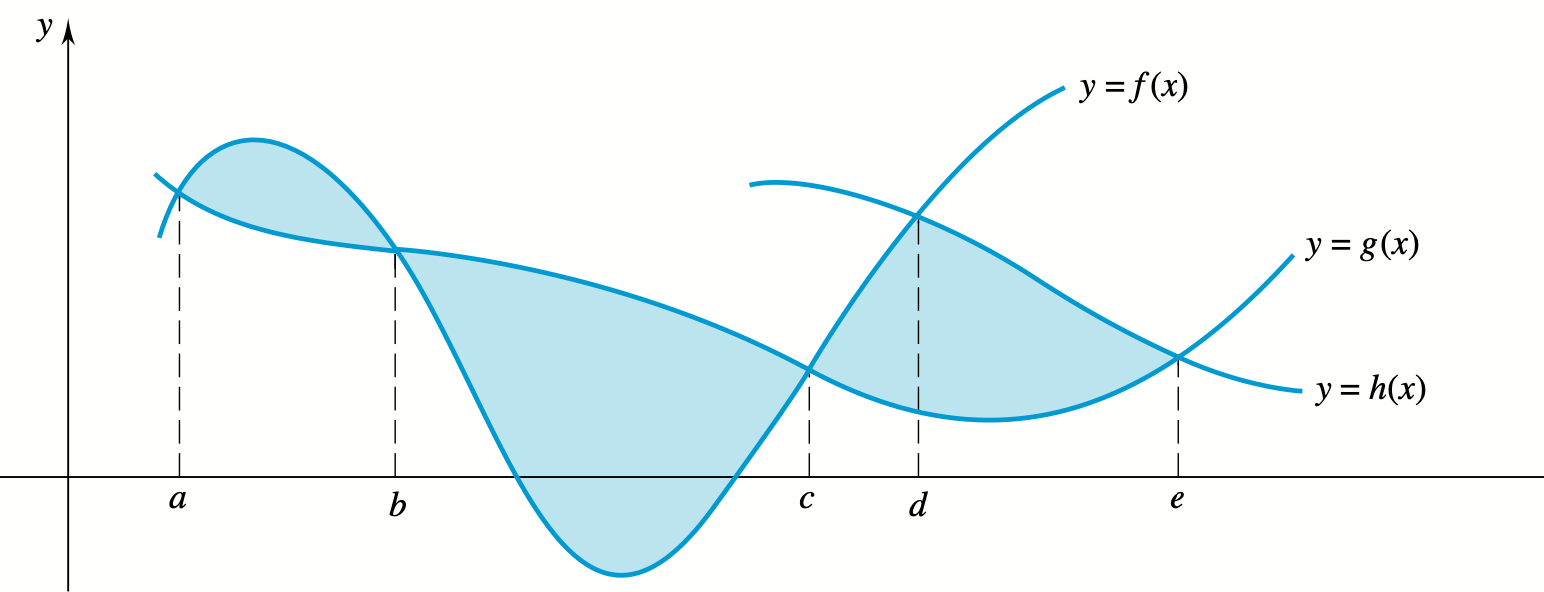
\includegraphics[height=.28\textwidth]{pics/areas-7c.png}
\end{center}
